\chapter{Marco Teórico}

\section{¿Qué es un Sistema Operativo?}

Un sistema operativo es un software que gestiona los recursos de hardware y coordina la ejecución de programas en un sistema informático. Está compuesto por un conjunto de programas de propósito específico que permiten el correcto funcionamiento del equipo. Entre sus funciones principales se encuentran la gestión de archivos y carpetas, el control de periféricos, la administración de memoria y la interacción con el usuario \parencite{ibm_que_es_so}.

\section{Tipos de sistema}

Los sistemas operativos pueden clasificarse según el tipo de hardware y las funciones que desempeñan \parencite{iglesiasconceptos}. A continuación, se detallan las categorías más relevantes.

\subsection{Según el número de usuarios}
\begin{itemize}
    \item \textbf{Monotarea:} sistema operativo que permite ejecutar únicamente los programas de un usuario en un momento dado.
    \item \textbf{Multiusuario:} sistema operativo que admite la ejecución simultánea de programas de varios usuarios, garantizando aislamiento entre ellos.
\end{itemize}

\subsection{Según la gestión de tareas}
\begin{itemize}
    \item \textbf{Monotarea:} un sistema que solo admite la ejecución de un proceso a la vez, limitando la concurrencia en el equipo.
    \item \textbf{Multitarea:} permite ejecutar varios procesos de manera concurrente; por ejemplo, mientras un usuario navega en Internet, el sistema puede reproducir música en segundo plano \textcite{ibm_que_es_so}.
\end{itemize}

\subsection{Sistemas operativos en tiempo real (RTOS)}

Los sistemas en tiempo real se distinguen por dos propiedades: \textbf{predictibilidad} y \textbf{determinismo}. Estas características permiten garantizar que ciertas operaciones críticas se ejecuten en intervalos de tiempo definidos \parencite{windriver_rtos}. Se diferencian dos tipos: los de \textit{tiempo real duro}, en los cuales un fallo en el tiempo de respuesta es crítico, y los de \textit{tiempo real blando}, donde la puntualidad es deseable pero no esencial.

\subsection{Sistemas operativos distribuidos}

Un sistema distribuido permite ejecutar procesos en múltiples ordenadores de manera coordinada. Estos sistemas comparten recursos de diferentes máquinas y ofrecen al usuario una interfaz unificada, de modo que no percibe la distribución física de los recursos. Para lograrlo, el sistema operativo se encarga de gestionar la comunicación, la sincronización y el intercambio de datos entre nodos \textcite{ibm_que_es_so}.

\subsection{Sistemas operativos móviles}

Los sistemas operativos móviles permiten que dispositivos como teléfonos inteligentes y tabletas ejecuten aplicaciones. Actúan como intermediarios entre los componentes de hardware y las aplicaciones de software, facilitando la interacción del usuario con el dispositivo \parencite{techtarget_os_definition}.

\subsection{Sistemas operativos embebidos}

Los sistemas operativos embebidos se diseñan para administrar recursos en dispositivos especializados, como automóviles, electrodomésticos o sistemas de control industrial. Estos sistemas priorizan la eficiencia y la confiabilidad, dado que suelen operar en entornos con recursos limitados \textcite{ibm_que_es_so}.

\section{Arquitecturas de los sistemas operativos}

El núcleo (\textit{kernel}) constituye la parte esencial del sistema operativo, encargado de gestionar los recursos del hardware y de proporcionar los servicios fundamentales a las aplicaciones. Se identifican tres enfoques arquitectónicos principales: el \textbf{monolítico}, el \textbf{microkernel} y el \textbf{híbrido}, cada uno con ventajas y desventajas en términos de rendimiento, estabilidad y complejidad \parencite{barbadekar2023}.

\subsection{Kernel monolítico}

En este modelo, todos los servicios del sistema operativo como controladores de dispositivos, sistemas de archivos y protocolos de red se ejecutan en el espacio del núcleo. \textcite{barbadekar2023} explican que esta integración favorece la eficiencia y el rendimiento, aunque conlleva una mayor complejidad y menor flexibilidad a la hora de extender o modificar el sistema.

\begin{figure}[H]
  \centering
  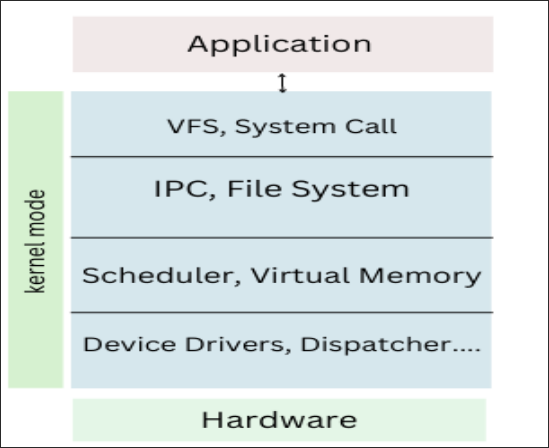
\includegraphics[width=0.75\textwidth]{figures/monolithic.png}
  \caption[Kernel monolítico]%
  {Esquema de arquitectura de un kernel monolítico. Extraído de \parencite{barbadekar2023}.}
  \label{fig:monolithic}
\end{figure}

\subsection{Microkernel}

El enfoque de microkernel sigue el principio de minimalismo: únicamente las funciones esenciales (gestión de memoria, planificación e intercomunicación entre procesos) se implementan en el núcleo, mientras que otros servicios se ejecutan en espacio de usuario. Esto reduce la superficie de ataque y mejora la estabilidad, pero introduce sobrecarga en las comunicaciones entre procesos, afectando al rendimiento \parencite{barbadekar2023}.


\begin{figure}[htbp]
  \centering
  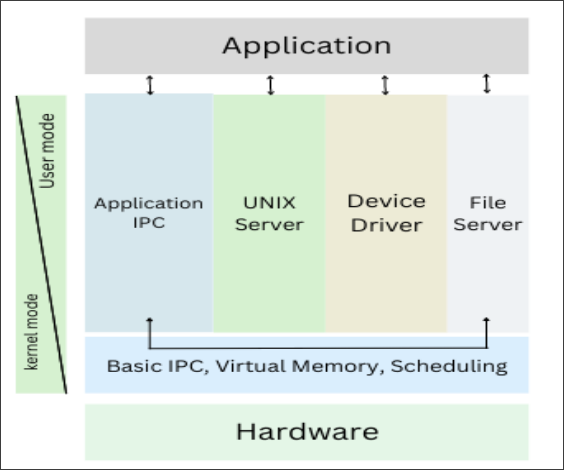
\includegraphics[width=0.75\textwidth]{figures/microkernel.png}
  \caption[Microkernel]{Arquitectura de microkernel. Extraído de \parencite{barbadekar2023}.}
  \label{fig:microkernel}
\end{figure}


\subsection{Kernel híbrido}

El kernel híbrido busca equilibrar los dos modelos anteriores. \textcite{barbadekar2023} destacan que combina la separación modular del microkernel con la eficiencia del monolítico, de modo que ciertos servicios permanecen en el espacio del núcleo mientras otros se gestionan en el espacio de usuario. Con ello se obtiene una arquitectura más flexible que optimiza tanto el rendimiento como la seguridad y la estabilidad del sistema.

\begin{figure}[htbp]
  \centering
  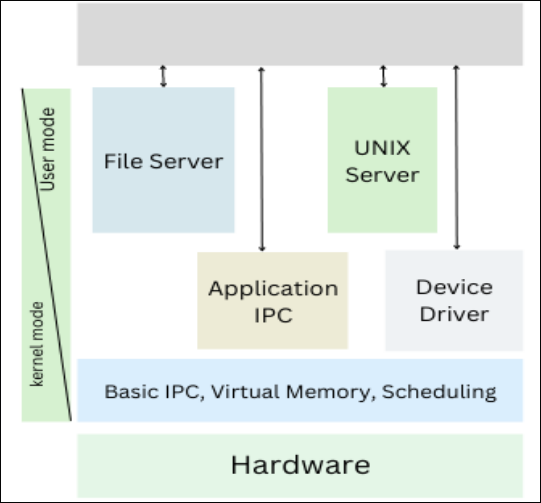
\includegraphics[width=0.75\textwidth]{figures/hybrid.png}
  \caption[Kernel híbrido] {Arquitectura de un kernel híbrido. Extraído de \parencite{barbadekar2023}.}
  \label{fig:hybrid}
\end{figure}

\subsection{Comparativa de las arquitecturas de los sistemas operativos}



\begin{table}[H]
\centering
\begin{tabular}{p{2.8cm}p{3.5cm}p{3.5cm}p{3.5cm}}
\hline
\textbf{Parámetro de desempeño} & \textbf{Kernel monolítico} & \textbf{Microkernel} & \textbf{Kernel híbrido} \\
\hline
Eficiencia & Operación más eficiente ya que todos los componentes están integrados & Bajo sobrecosto y alta eficiencia & Conocido por su operación eficiente \\
\hline
Complejidad & Más complejo & Menos complejo & Menos complejo \\
\hline
Estabilidad & Menos estable & Menor estabilidad y confiabilidad & Más estable \\
\hline
Seguridad & Menos seguro & Más seguro que los monolíticos tradicionales & Más seguro \\
\hline
Velocidad & Más rápido en términos de rendimiento del sistema al integrar todos los componentes & Mayor rendimiento & Más lento que un kernel monolítico puro, pero más rápido que un microkernel puro \\
\hline
\end{tabular}
\caption[Comparaci\'on entre arquitecturas de sistemas operativos]{Comparaci\'on entre arquitecturas de sistemas operativos. Adaptado de \parencite{barbadekar2023}.}
\label{tab:comparacion-kernels}
\end{table}

